\documentclass[12pt,a4paper]{article}
\usepackage[utf8]{inputenc}
\usepackage[T1]{fontenc}
\usepackage[english]{babel}
\usepackage{fancyhdr}
\usepackage{kpfonts}
\usepackage[margin=1in]{geometry}
\usepackage{exsheets}
\usepackage{amsmath, amssymb, amsfonts}
\usepackage{enumerate}
\usepackage{tikz}
\usepackage{tabularx}
\usetikzlibrary{arrows, decorations.text}

\pagestyle{fancy}
\renewcommand{\headrulewidth}{2pt}
\fancyhead[L]{EPITA\_ING1\_BING\_2020\_S6\_PARTIEL\_GREF}
\fancyhead[R]{June 2018}

\fancyfoot[C]{\textbf{\thepage}}
\fancyfoot[L]{}

\SetupExSheets{solution/print=true}
\SetupExSheets{question/type=exam}
\SetupExSheets[points]{name=point,name-plural=points}
\RenewQuSolPair{question}[name={\large Exercise}]{solution}

\begin{document}
\begin{center}

  {\Large \textbf{Networks and Flows on Graphs\footnote{Head of course : P.~Siarry.}}}\\

  \vspace{10pt}
  {\Large \textit{Final Exam}}

  \vspace{2\baselineskip}
\end{center}
\begin{center}
\begin{minipage}{\textwidth}
  Duration of the exam : 1h30\\
  No documents are allowed\\
  Only \emph{non-programmable} pocket calculators are allowed\\
  Exercises can be done independently.
\end{minipage}
\end{center}
\rule{\textwidth}{2pt}


\vspace{\baselineskip}

\begin{question}
  Exploiting a newly found mineral deposit involves the execution of
  hereby listed tasks. Table features each tasks identifier,
  description, duration and prior tasks.

    \vspace{2\baselineskip}
  \begin{center}
    \renewcommand{\arraystretch}{1.5}
    \begin{tabularx}{\textwidth}{|c|p{6.75cm}|c|c|}
      \hline
      Label of task & Task description & Time (in weeks)  & Prior Tasks\\
      \hline
      A  & Obtainging construction permit & 120 & --   \\
      \hline
      B  & Setting up a 6 km track & 180 & A  \\
      \hline
      C  & Installation of two drill machines & 3 & B  \\
      \hline
      D  & Setting temporary offices for mapping team and lodging for drilling one & 30 & B  \\
      \hline
      E  & Tarmac the track & 60 & B  \\
      \hline
      F  & Water conveyance & 90 & D  \\
      \hline
      G  & Probing phase & 240 & C, D  \\
      \hline
      H  & Drilling and equipping three wells & 180 & E, F, G  \\
      \hline
      I  & Installing exploiting equipment down the wells & 30 & J, H  \\
      \hline
      J  & Setting up pemanent offices and lodgings for engineers and workers & 240 & E, F, G  \\
      \hline
      K  & Tracing and layout of galleries & 360 & J, H  \\
      \hline
      L  & Setting up washing system & 240 & J, H  \\
      \hline
    \end{tabularx}
  \end{center}
  \vspace{\baselineskip}
  \begin{enumerate}
  \item Draw the MPM (Meta Potential Model) graph of this project
    planning problem.
  \item Using relevant algorithms, give earliest scheduling dates.
    \begin{itemize}
    \item What is the minimum amount of time the project needs to be done?
    \item What are the critical tasks?
    \end{itemize}
  \item Using relevant algorithms, give latest scheduling dates.
    \begin{itemize}
    \item What is the total margin of the project? Compute free
      margins of non-critical tasks?
    \end{itemize}
  \end{enumerate}
\end{question}
\begin{question}
  Using Floyd-Warshall's algorithm, compute all minimal paths between
  any two pairs of vertices of the following graph. Could we look for
  all maximal paths between any such pairs?  \vspace{2\baselineskip}
  \begin{center}
    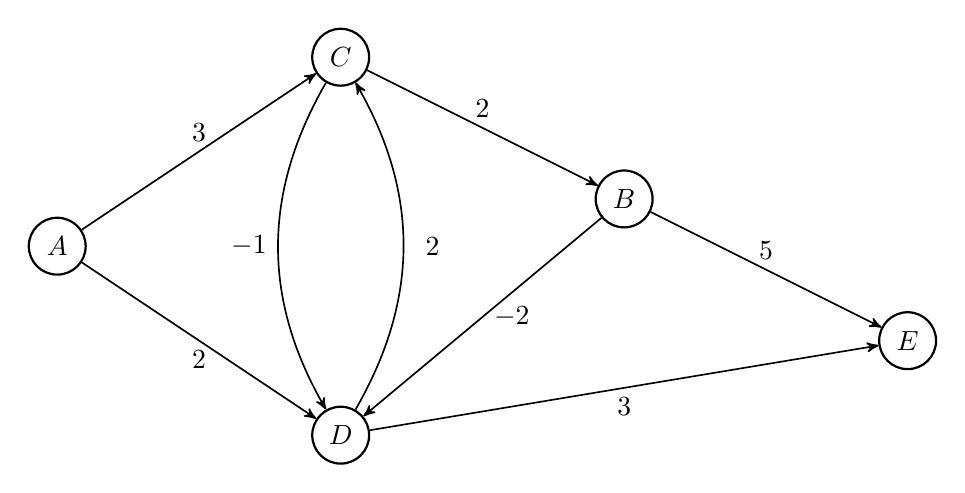
\begin{tikzpicture}
      [minimum width={width("b")+1.5em},
      vertex/.style={circle, draw=black, fill=white, thick},
      arr/.style={->,>=stealth',semithick},
      scale=1.2]
      \node (E) at (10, 5) [vertex] {$E$};
      \node (D) at (4, 4) [vertex] {$D$}
      edge[arr] node[below] {$3$} (E);
      \node (B) at (7, 6.5) [vertex] {$B$}
      edge[arr] node[above] {$5$} (E)
      edge[arr] node[right] {$-2$} (D);
      \node (C) at (4, 8) [vertex] {$C$}
      edge[arr, bend right] node[left] {$-1$} (D)
      edge[arr] node[above] {$2$} (B);
      \node (A) at (1, 6) [vertex] {$A$}
      edge[arr] node[above] {$3$} (C)
      edge[arr] node[below] {$2$} (D);
      \path (D) edge[arr, bend right] node[right] {$2$} (C);
    \end{tikzpicture}
  \end{center}
  \vspace{2\baselineskip}
\end{question}
\end{document}

%%% Local Variables:
%%% mode: latex
%%% TeX-master: t
%%% End:
